\documentclass[10pt]{article}
% Shared preamble: Nature-style article layout (single column, sans headings,
% superscript numbered references, "Fig. 1 |" captions).
\usepackage[a4paper,top=2.2cm,bottom=2.4cm,left=2.4cm,right=2.4cm]{geometry}
\usepackage[T1]{fontenc}
\usepackage[utf8]{inputenc}
\usepackage{newtxtext,newtxmath}
\usepackage[scaled=0.92]{helvet}
\usepackage{microtype}
\usepackage{graphicx}
\usepackage{booktabs,tabularx,multirow,makecell,threeparttable,longtable,array}
\usepackage[table]{xcolor}
\usepackage{siunitx}
\sisetup{group-separator={,},group-minimum-digits=4,detect-all,per-mode=symbol}
\usepackage{amsmath,bm}
\usepackage[version=4]{mhchem}
\usepackage{caption}
\usepackage{titlesec}
\usepackage{enumitem}
\usepackage{fancyhdr}
\usepackage{placeins}
\usepackage{float}
\usepackage{ragged2e}

\definecolor{natureblue}{HTML}{1C5CAB}
\definecolor{inkgray}{HTML}{52514E}

% ---- References: Nature style (biblatex-nature), superscript citations
\usepackage[super,sort&compress,comma]{natbib}
\renewcommand{\bibfont}{\small}
\setlength{\bibsep}{1pt}
\providecommand{\urlprefix}{}
\usepackage{url}

\usepackage[colorlinks=true,linkcolor=natureblue,citecolor=natureblue,
            urlcolor=natureblue,pdfusetitle]{hyperref}

% ---- Headings: bold sans, unnumbered, Nature-like
\titleformat{\section}{\sffamily\bfseries\large}{}{0pt}{}
\titleformat{\subsection}{\sffamily\bfseries\normalsize}{}{0pt}{}
\titleformat{\subsubsection}[runin]{\sffamily\bfseries\normalsize}{}{0pt}{}[.]
\titlespacing*{\section}{0pt}{14pt}{6pt}
\titlespacing*{\subsection}{0pt}{10pt}{3pt}
\titlespacing*{\subsubsection}{0pt}{6pt}{0.6em}
\setcounter{secnumdepth}{0}

% ---- Captions: "Fig. 1 | Title. Legend." in small sans
\DeclareCaptionLabelSeparator{nature}{\,\textbar\,\,}
\captionsetup{font={small,sf},labelfont={bf,sf},labelsep=nature,justification=justified,
              singlelinecheck=false,skip=4pt}
\captionsetup[figure]{name=Fig.}
\captionsetup[table]{name=Table,position=top}

% ---- Misc
\setlength{\parskip}{0pt}
\setlength{\parindent}{1.2em}
\linespread{1.08}
\setlist{nosep,leftmargin=1.4em}
\renewcommand{\arraystretch}{1.12}
\newcommand{\COtwoe}{CO\textsubscript{2}e}
\newcommand{\COtwo}{CO\textsubscript{2}}
\newcommand{\CHfour}{CH\textsubscript{4}}
\newcommand{\NtwoO}{N\textsubscript{2}O}
\newcommand{\figref}[1]{Fig.~\ref{#1}}
\newcommand{\edfigref}[1]{Extended Data Fig.~\ref{#1}}
\newcommand{\edtabref}[1]{Extended Data Table~\ref{#1}}
\newcommand{\sinote}[1]{Supplementary Note~#1}

\pagestyle{fancy}
\fancyhf{}
\renewcommand{\headrulewidth}{0pt}
\fancyfoot[C]{\sffamily\footnotesize\thepage}

% Auto-generated by scripts/run_all.py -- do not edit by hand.
\newcommand{\ArSixDelta}{2.9}
\newcommand{\BasketEqFishDesc}{103\,g lentils, 77\,g kidney beans, 76\,g salmon, 0.5 zinc tablet, 0.2 b12 tablet}
\newcommand{\BasketEqFishEnergy}{1.6}
\newcommand{\BasketEqFishGhg}{1.58}
\newcommand{\BasketEqFishKcal}{374}
\newcommand{\BasketEqFishMass}{256}
\newcommand{\BasketEqFishReduction}{72}
\newcommand{\BasketEqFishShort}{all key nutrients matched}
\newcommand{\BasketEqMeatDesc}{118\,g chickpeas, 54\,g chicken breast, 51\,g lentils, 4\,g mycoprotein, 0.4 zinc tablet, 0.3 b12 tablet}
\newcommand{\BasketEqMeatEnergy}{1.5}
\newcommand{\BasketEqMeatGhg}{0.97}
\newcommand{\BasketEqMeatKcal}{347}
\newcommand{\BasketEqMeatMass}{228}
\newcommand{\BasketEqMeatReduction}{83}
\newcommand{\BasketEqMeatShort}{all key nutrients matched}
\newcommand{\BasketEqVeganDesc}{126\,g kidney beans, 98\,g mycoprotein, 65\,g chickpeas, 0.3 b12 tablet, 0.1 zinc tablet}
\newcommand{\BasketEqVeganEnergy}{1.6}
\newcommand{\BasketEqVeganGhg}{0.36}
\newcommand{\BasketEqVeganKcal}{363}
\newcommand{\BasketEqVeganMass}{290}
\newcommand{\BasketEqVeganReduction}{93}
\newcommand{\BasketEqVeganShort}{all key nutrients matched}
\newcommand{\BasketEqVegetarianDesc}{184\,g kidney beans, 112\,g egg, 0.4 zinc tablet, 0.3 b12 tablet}
\newcommand{\BasketEqVegetarianEnergy}{1.8}
\newcommand{\BasketEqVegetarianGhg}{0.81}
\newcommand{\BasketEqVegetarianKcal}{407}
\newcommand{\BasketEqVegetarianMass}{296}
\newcommand{\BasketEqVegetarianReduction}{86}
\newcommand{\BasketEqVegetarianShort}{all key nutrients matched}
\newcommand{\BasketMeatSwapDesc}{171\,g chicken breast, 85\,g pork loin}
\newcommand{\BasketMeatSwapEnergy}{2.0}
\newcommand{\BasketMeatSwapGhg}{4.02}
\newcommand{\BasketMeatSwapKcal}{460}
\newcommand{\BasketMeatSwapMass}{256}
\newcommand{\BasketMeatSwapReduction}{28}
\newcommand{\BasketMeatSwapShort}{vitamin B\textsubscript{12} short by 57\%}
\newcommand{\BasketOmnivoreDesc}{300\,g milk, 140\,g lentils, 85\,g mycoprotein, 12\,g salmon, 11\,g fortified cereal}
\newcommand{\BasketOmnivoreEnergy}{2.0}
\newcommand{\BasketOmnivoreGhg}{1.59}
\newcommand{\BasketOmnivoreKcal}{460}
\newcommand{\BasketOmnivoreMass}{548}
\newcommand{\BasketOmnivoreReduction}{71}
\newcommand{\BasketOmnivoreShort}{vitamin B\textsubscript{12} short by 23\%}
\newcommand{\BasketVeganFortifiedDesc}{300\,g soy drink, 94\,g mycoprotein, 29\,g pumpkin seeds, 20\,g fortified cereal, 5\,g lentils}
\newcommand{\BasketVeganFortifiedEnergy}{2.0}
\newcommand{\BasketVeganFortifiedGhg}{0.69}
\newcommand{\BasketVeganFortifiedKcal}{460}
\newcommand{\BasketVeganFortifiedMass}{448}
\newcommand{\BasketVeganFortifiedReduction}{88}
\newcommand{\BasketVeganFortifiedShort}{vitamin B\textsubscript{12} short by 54\%}
\newcommand{\BasketVeganWholefoodDesc}{116\,g mycoprotein, 95\,g kidney beans, 81\,g lentils}
\newcommand{\BasketVeganWholefoodEnergy}{1.4}
\newcommand{\BasketVeganWholefoodGhg}{0.38}
\newcommand{\BasketVeganWholefoodKcal}{328}
\newcommand{\BasketVeganWholefoodMass}{292}
\newcommand{\BasketVeganWholefoodReduction}{93}
\newcommand{\BasketVeganWholefoodShort}{vitamin B\textsubscript{12} short by 100\%}
\newcommand{\BasketVegetarianDesc}{300\,g milk, 148\,g lentils, 112\,g soy drink, 84\,g mycoprotein, 3\,g fortified cereal}
\newcommand{\BasketVegetarianEnergy}{2.0}
\newcommand{\BasketVegetarianGhg}{1.46}
\newcommand{\BasketVegetarianKcal}{460}
\newcommand{\BasketVegetarianMass}{646}
\newcommand{\BasketVegetarianReduction}{74}
\newcommand{\BasketVegetarianShort}{vitamin B\textsubscript{12} short by 24\%}
\newcommand{\BeefBtwelve}{2.80}
\newcommand{\BeefBtwelveAbs}{1.68}
\newcommand{\BeefGasChFour}{55}
\newcommand{\BeefGasCoTwo}{24}
\newcommand{\BeefGasNTwoo}{21}
\newcommand{\BeefIron}{3.08}
\newcommand{\BeefIronAbs}{0.61}
\newcommand{\BeefKcal}{230}
\newcommand{\BeefPcKg}{384}
\newcommand{\BeefPcT}{0.38}
\newcommand{\BeefProtein}{28.4}
\newcommand{\BeefProteinQ}{28.1}
\newcommand{\BeefSatfat}{4.7}
\newcommand{\BeefSelenium}{21.6}
\newcommand{\BeefSodium}{87}
\newcommand{\BeefZinc}{6.84}
\newcommand{\BeefZincAbs}{2.39}
\newcommand{\BenefitTotal}{£41k (£21k--68k)}
\newcommand{\BreakEvenLossMeal}{0.52}
\newcommand{\CampusBeefMeals}{79{,}000}
\newcommand{\CampusBeefT}{9.5}
\newcommand{\CampusEfConseq}{31.0}
\newcommand{\CampusLrAcct}{232}
\newcommand{\CampusLrAcctHi}{314}
\newcommand{\CampusLrAcctLo}{165}
\newcommand{\CampusLrGross}{293}
\newcommand{\CampusLrGrossHi}{373}
\newcommand{\CampusLrGrossLo}{233}
\newcommand{\CampusLrLeak}{61}
\newcommand{\CampusLrLeakHi}{109}
\newcommand{\CampusLrLeakLo}{35}
\newcommand{\CampusLrNet}{150}
\newcommand{\CampusLrNetHi}{223}
\newcommand{\CampusLrNetLo}{83}
\newcommand{\CampusLrOff}{17}
\newcommand{\CampusLrOffHi}{51}
\newcommand{\CampusLrOffLo}{3}
\newcommand{\CampusLrSubs}{65}
\newcommand{\CampusLrSubsAdj}{6}
\newcommand{\CampusLrSubsAdjHi}{14}
\newcommand{\CampusLrSubsAdjLo}{0}
\newcommand{\CampusLrSubsHi}{103}
\newcommand{\CampusLrSubsLo}{42}
\newcommand{\CampusNetVsAcctLr}{65}
\newcommand{\CampusNetVsAcctSr}{20}
\newcommand{\CampusNetVsGrossLr}{52}
\newcommand{\CampusNoResponse}{65}
\newcommand{\CampusPassLr}{0.78}
\newcommand{\CampusPassSr}{0.28}
\newcommand{\CampusPctCatering}{7}
\newcommand{\CampusPctImperial}{0.06}
\newcommand{\CampusPeople}{32{,}861}
\newcommand{\CampusPhiStar}{0.25}
\newcommand{\CampusPpmLondon}{5.2}
\newcommand{\CampusProbIncreaseSr}{0.6}
\newcommand{\CampusSrAcct}{233}
\newcommand{\CampusSrAcctHi}{316}
\newcommand{\CampusSrAcctLo}{166}
\newcommand{\CampusSrGross}{294}
\newcommand{\CampusSrGrossHi}{374}
\newcommand{\CampusSrGrossLo}{233}
\newcommand{\CampusSrLeak}{197}
\newcommand{\CampusSrLeakHi}{261}
\newcommand{\CampusSrLeakLo}{148}
\newcommand{\CampusSrNet}{47}
\newcommand{\CampusSrNetHi}{88}
\newcommand{\CampusSrNetLo}{15}
\newcommand{\CampusSrOff}{18}
\newcommand{\CampusSrOffHi}{51}
\newcommand{\CampusSrOffLo}{3}
\newcommand{\CampusSrSubs}{64}
\newcommand{\CampusSrSubsAdj}{36}
\newcommand{\CampusSrSubsAdjHi}{63}
\newcommand{\CampusSrSubsAdjLo}{21}
\newcommand{\CampusSrSubsHi}{103}
\newcommand{\CampusSrSubsLo}{41}
\newcommand{\CarbonValue}{277}
\newcommand{\CarbonValueHigh}{416}
\newcommand{\CarbonValueLow}{139}
\newcommand{\Cbe}{88.0}
\newcommand{\CbeFood}{9.8}
\newcommand{\CocLondonMt}{21}
\newcommand{\CocPerKg}{144}
\newcommand{\CookYield}{0.69}
\newcommand{\CostPerT}{£1{,}730 (£911--3{,}725)}
\newcommand{\CostPerTCapped}{£1{,}444}
\newcommand{\CumGwpHundredFifty}{142}
\newcommand{\CumGwpHundredHundred}{284}
\newcommand{\CumGwpHundredTwenty}{57}
\newcommand{\CumStarFifty}{232}
\newcommand{\CumStarHundred}{308}
\newcommand{\CumStarRatioFifty}{1.6}
\newcommand{\CumStarRatioHundred}{1.1}
\newcommand{\CumStarRatioTwenty}{3.3}
\newcommand{\CumStarTwenty}{186}
\newcommand{\CweKg}{15.8}
\newcommand{\DeltaBtwelveMeal}{1.4}
\newcommand{\DeltaFibreMeal}{3.0}
\newcommand{\DeltaIronAbsMeal}{0.21}
\newcommand{\DeltaIronMeal}{0.42}
\newcommand{\DeltaKcalMeal}{29}
\newcommand{\DeltaPcEqFish}{275}
\newcommand{\DeltaPcEqMeat}{317}
\newcommand{\DeltaPcEqVegan}{359}
\newcommand{\DeltaPcEqVegetarian}{328}
\newcommand{\DeltaProteinMeal}{2.0}
\newcommand{\DeltaZincAbsMeal}{1.08}
\newcommand{\DeltaZincMeal}{2.7}
\newcommand{\DishEps}{1.5}
\newcommand{\EfBeefPnHerd}{99.5}
\newcommand{\EfBeefPnMix}{66.4}
\newcommand{\EfBeefPnUk}{37.1}
\newcommand{\EfBeefUkAttr}{34.7}
\newcommand{\EfBeefUkConseq}{31.0}
\newcommand{\EqBeansAll}{never}
\newcommand{\EqBeansBinding}{vitamin B\textsubscript{12}}
\newcommand{\EqBeansBtwelve}{never}
\newcommand{\EqBeansIron}{207\,g}
\newcommand{\EqBeansProtein}{369\,g}
\newcommand{\EqBeansSelenium}{1.8\,kg}
\newcommand{\EqBeansZinc}{1.2\,kg}
\newcommand{\EqCerealAll}{never}
\newcommand{\EqCerealBinding}{vitamin B6}
\newcommand{\EqCerealBtwelve}{160\,g}
\newcommand{\EqCerealIron}{76\,g}
\newcommand{\EqCerealProtein}{625\,g}
\newcommand{\EqCerealSelenium}{never}
\newcommand{\EqCerealZinc}{383\,g}
\newcommand{\EqCheddarAll}{11.5\,kg}
\newcommand{\EqCheddarBinding}{niacin}
\newcommand{\EqCheddarBtwelve}{235\,g}
\newcommand{\EqCheddarIron}{4.3\,kg}
\newcommand{\EqCheddarProtein}{123\,g}
\newcommand{\EqCheddarSelenium}{76\,g}
\newcommand{\EqCheddarZinc}{188\,g}
\newcommand{\EqChickenAll}{824\,g}
\newcommand{\EqChickenBinding}{vitamin B\textsubscript{12}}
\newcommand{\EqChickenBtwelve}{824\,g}
\newcommand{\EqChickenIron}{349\,g}
\newcommand{\EqChickenProtein}{91\,g}
\newcommand{\EqChickenSelenium}{78\,g}
\newcommand{\EqChickenZinc}{684\,g}
\newcommand{\EqChickpeasAll}{never}
\newcommand{\EqChickpeasBinding}{vitamin B\textsubscript{12}}
\newcommand{\EqChickpeasBtwelve}{never}
\newcommand{\EqChickpeasIron}{210\,g}
\newcommand{\EqChickpeasProtein}{418\,g}
\newcommand{\EqChickpeasSelenium}{584\,g}
\newcommand{\EqChickpeasZinc}{869\,g}
\newcommand{\EqEggAll}{10.6\,kg}
\newcommand{\EqEggBinding}{niacin}
\newcommand{\EqEggBtwelve}{1.7\,kg}
\newcommand{\EqEggIron}{511\,g}
\newcommand{\EqEggProtein}{223\,g}
\newcommand{\EqEggSelenium}{70\,g}
\newcommand{\EqEggZinc}{651\,g}
\newcommand{\EqLentilsAll}{never}
\newcommand{\EqLentilsBinding}{vitamin B\textsubscript{12}}
\newcommand{\EqLentilsBtwelve}{never}
\newcommand{\EqLentilsIron}{183\,g}
\newcommand{\EqLentilsProtein}{537\,g}
\newcommand{\EqLentilsSelenium}{771\,g}
\newcommand{\EqLentilsZinc}{1.0\,kg}
\newcommand{\EqMilkAll}{30.4\,kg}
\newcommand{\EqMilkBinding}{iron}
\newcommand{\EqMilkBtwelve}{488\,g}
\newcommand{\EqMilkIron}{30.4\,kg}
\newcommand{\EqMilkProtein}{852\,g}
\newcommand{\EqMilkSelenium}{864\,g}
\newcommand{\EqMilkZinc}{1.4\,kg}
\newcommand{\EqMycoproteinAll}{never}
\newcommand{\EqMycoproteinBinding}{vitamin B\textsubscript{12}}
\newcommand{\EqMycoproteinBtwelve}{never}
\newcommand{\EqMycoproteinIron}{1.2\,kg}
\newcommand{\EqMycoproteinProtein}{196\,g}
\newcommand{\EqMycoproteinSelenium}{120\,g}
\newcommand{\EqMycoproteinZinc}{137\,g}
\newcommand{\EqOatsAll}{never}
\newcommand{\EqOatsBinding}{vitamin B\textsubscript{12}}
\newcommand{\EqOatsBtwelve}{never}
\newcommand{\EqOatsIron}{143\,g}
\newcommand{\EqOatsProtein}{374\,g}
\newcommand{\EqOatsSelenium}{75\,g}
\newcommand{\EqOatsZinc}{365\,g}
\newcommand{\EqPeaMinceAll}{never}
\newcommand{\EqPeaMinceBinding}{iron}
\newcommand{\EqPeaMinceBtwelve}{never}
\newcommand{\EqPeaMinceIron}{never}
\newcommand{\EqPeaMinceProtein}{241\,g}
\newcommand{\EqPeaMinceSelenium}{never}
\newcommand{\EqPeaMinceZinc}{never}
\newcommand{\EqPeanutsAll}{never}
\newcommand{\EqPeanutsBinding}{vitamin B\textsubscript{12}}
\newcommand{\EqPeanutsBtwelve}{never}
\newcommand{\EqPeanutsIron}{385\,g}
\newcommand{\EqPeanutsProtein}{268\,g}
\newcommand{\EqPeanutsSelenium}{232\,g}
\newcommand{\EqPeanutsZinc}{480\,g}
\newcommand{\EqPeasAll}{never}
\newcommand{\EqPeasBinding}{vitamin B\textsubscript{12}}
\newcommand{\EqPeasBtwelve}{never}
\newcommand{\EqPeasIron}{400\,g}
\newcommand{\EqPeasProtein}{803\,g}
\newcommand{\EqPeasSelenium}{2.2\,kg}
\newcommand{\EqPeasZinc}{2.0\,kg}
\newcommand{\EqPorkAll}{384\,g}
\newcommand{\EqPorkBinding}{vitamin B\textsubscript{12}}
\newcommand{\EqPorkBtwelve}{384\,g}
\newcommand{\EqPorkIron}{306\,g}
\newcommand{\EqPorkProtein}{98\,g}
\newcommand{\EqPorkSelenium}{62\,g}
\newcommand{\EqPorkZinc}{270\,g}
\newcommand{\EqSalmonAll}{1.6\,kg}
\newcommand{\EqSalmonBinding}{zinc}
\newcommand{\EqSalmonBtwelve}{143\,g}
\newcommand{\EqSalmonIron}{1.2\,kg}
\newcommand{\EqSalmonProtein}{127\,g}
\newcommand{\EqSalmonSelenium}{52\,g}
\newcommand{\EqSalmonZinc}{1.6\,kg}
\newcommand{\EqSeedsAll}{never}
\newcommand{\EqSeedsBinding}{vitamin B\textsubscript{12}}
\newcommand{\EqSeedsBtwelve}{never}
\newcommand{\EqSeedsIron}{69\,g}
\newcommand{\EqSeedsProtein}{155\,g}
\newcommand{\EqSeedsSelenium}{230\,g}
\newcommand{\EqSeedsZinc}{170\,g}
\newcommand{\EqSoyDrinkAll}{3.7\,kg}
\newcommand{\EqSoyDrinkBinding}{zinc}
\newcommand{\EqSoyDrinkBtwelve}{884\,g}
\newcommand{\EqSoyDrinkIron}{1.4\,kg}
\newcommand{\EqSoyDrinkProtein}{897\,g}
\newcommand{\EqSoyDrinkSelenium}{939\,g}
\newcommand{\EqSoyDrinkZinc}{3.7\,kg}
\newcommand{\EqTofuAll}{never}
\newcommand{\EqTofuBinding}{vitamin B\textsubscript{12}}
\newcommand{\EqTofuBtwelve}{never}
\newcommand{\EqTofuIron}{229\,g}
\newcommand{\EqTofuProtein}{168\,g}
\newcommand{\EqTofuSelenium}{124\,g}
\newcommand{\EqTofuZinc}{610\,g}
\newcommand{\EqVenisonAll}{210\,g}
\newcommand{\EqVenisonBinding}{selenium}
\newcommand{\EqVenisonBtwelve}{121\,g}
\newcommand{\EqVenisonIron}{92\,g}
\newcommand{\EqVenisonProtein}{106\,g}
\newcommand{\EqVenisonSelenium}{210\,g}
\newcommand{\EqVenisonZinc}{132\,g}
\newcommand{\FlowCwe}{15.8}
\newcommand{\FlowEaten}{6.9}
\newcommand{\FlowEatenGDay}{19}
\newcommand{\FlowRetail}{11.1}
\newcommand{\FoiBeefTwentyFour}{0.07}
\newcommand{\FoiBeefTwentyThree}{8.5}
\newcommand{\FoiBeefTwentyTwo}{10.5}
\newcommand{\FoiChickenTwentyFour}{48.5}
\newcommand{\FoiChickenTwentyThree}{35.8}
\newcommand{\FoiChickenTwentyTwo}{23.8}
\newcommand{\FoiMeatTTwentyFour}{814}
\newcommand{\FoiMeatTTwentyThree}{929}
\newcommand{\FoiMeatTTwentyTwo}{907}
\newcommand{\FoiNarrative}{Beef purchases fell from 10.5\,t (2022/23) and 8.5\,t (2023/24) to 0.07\,t in 2024/25, while venison rose to 1.7\,t and pork and chicken purchases kept growing (to 15.6\,t and at least 48.5\,t). At this study's central emission factors the emissions embodied in meat purchases fell from 929\,t to 814\,t \COtwoe{} despite the growth in volume.}
\newcommand{\FoiPorkTwentyFour}{15.6}
\newcommand{\FoiPorkTwentyThree}{10.3}
\newcommand{\FoiPorkTwentyTwo}{8.3}
\newcommand{\FoiVenisonTwentyFour}{1.7}
\newcommand{\FoiVenisonTwentyThree}{1.6}
\newcommand{\FoiVenisonTwentyTwo}{0.0}
\newcommand{\FreqBtwelve}{27}
\newcommand{\FreqIronWomen}{0.8}
\newcommand{\FreqMeals}{2}
\newcommand{\FreqZincMen}{8}
\newcommand{\FreqZincWomen}{11}
\newcommand{\GwpTwentyDelta}{6.4}
\newcommand{\GwpTwentyFactor}{2.0}
\newcommand{\ImperialStaff}{8{,}941}
\newcommand{\ImperialStudents}{23{,}920}
\newcommand{\ImperialTotalKt}{247}
\newcommand{\Leggi}{28.61}
\newcommand{\LondonBeefMt}{3.49}
\newcommand{\LondonChFourKt}{68}
\newcommand{\LondonConseqDeltaEqFish}{2.13}
\newcommand{\LondonConseqDeltaEqMeat}{2.51}
\newcommand{\LondonConseqDeltaEqVegan}{2.89}
\newcommand{\LondonConseqDeltaEqVegetarian}{2.61}
\newcommand{\LondonDeltaEqFish}{2.50}
\newcommand{\LondonDeltaEqMeat}{2.88}
\newcommand{\LondonDeltaEqVegan}{3.26}
\newcommand{\LondonDeltaEqVegetarian}{2.98}
\newcommand{\LondonDeltaMax}{3.3}
\newcommand{\LondonDeltaMc}{2.8 (2.0--3.7)}
\newcommand{\LondonDeltaMcConseq}{2.4 (1.7--3.2)}
\newcommand{\LondonDeltaMin}{2.5}
\newcommand{\LondonDeltaPnMax}{6.4}
\newcommand{\LondonDeltaPnMin}{5.7}
\newcommand{\LondonPnDeltaEqFish}{5.69}
\newcommand{\LondonPnDeltaEqMeat}{6.07}
\newcommand{\LondonPnDeltaEqVegan}{6.45}
\newcommand{\LondonPnDeltaEqVegetarian}{6.17}
\newcommand{\LpEnergyMaxRatio}{2.0}
\newcommand{\LpEnergyTolHigh}{1.00}
\newcommand{\LpEnergyTolLow}{0.15}
\newcommand{\LpEnergyTolRelaxed}{2.00}
\newcommand{\LpEnergyTolStrict}{0.15}
\newcommand{\LpSatfatMaxRatio}{1.00}
\newcommand{\LpSodiumAllow}{150}
\newcommand{\MealPrice}{6.00}
\newcommand{\MealsM}{1.0}
\newcommand{\MinEnergyEqFish}{1.6}
\newcommand{\MinEnergyEqFishFeasible}{yes}
\newcommand{\MinEnergyEqMeat}{1.2}
\newcommand{\MinEnergyEqMeatFeasible}{yes}
\newcommand{\MinEnergyEqVegan}{1.3}
\newcommand{\MinEnergyEqVeganFeasible}{yes}
\newcommand{\MinEnergyEqVegetarian}{1.6}
\newcommand{\MinEnergyEqVegetarianFeasible}{yes}
\newcommand{\MinEnergyMeatSwap}{2.1}
\newcommand{\MinEnergyMeatSwapFeasible}{no}
\newcommand{\MinEnergyOmnivore}{2.3}
\newcommand{\MinEnergyOmnivoreFeasible}{yes}
\newcommand{\MinEnergyVeganFortified}{5.4}
\newcommand{\MinEnergyVeganFortifiedFeasible}{no}
\newcommand{\MinEnergyVeganWholefood}{1.4}
\newcommand{\MinEnergyVeganWholefoodFeasible}{no}
\newcommand{\MinEnergyVegetarian}{3.8}
\newcommand{\MinEnergyVegetarianFeasible}{no}
\newcommand{\NCampus}{4{,}000}
\newcommand{\NMC}{20{,}000}
\newcommand{\OutsideCost}{3.00}
\newcommand{\PBeefPct}{7.9}
\newcommand{\PaperAuthor}{F.~Song}
\newcommand{\PaperTitle}{Replacing beef: nutrition, emissions and the limits of a campus ban}
\newcommand{\PctCbeConseqEqFish}{2.4}
\newcommand{\PctCbeConseqEqMeat}{2.9}
\newcommand{\PctCbeConseqEqVegan}{3.3}
\newcommand{\PctCbeConseqEqVegetarian}{3.0}
\newcommand{\PctCbeEqFish}{2.8}
\newcommand{\PctCbeEqMeat}{3.3}
\newcommand{\PctCbeEqVegan}{3.7}
\newcommand{\PctCbeEqVegetarian}{3.4}
\newcommand{\PctCbeMax}{3.7}
\newcommand{\PctCbeMin}{2.8}
\newcommand{\PctCbePnEqFish}{6.5}
\newcommand{\PctCbePnEqMeat}{6.9}
\newcommand{\PctCbePnEqVegan}{7.3}
\newcommand{\PctCbePnEqVegetarian}{7.0}
\newcommand{\PctDiet}{16}
\newcommand{\PctLeggiConseqEqFish}{7.4}
\newcommand{\PctLeggiConseqEqMeat}{8.8}
\newcommand{\PctLeggiConseqEqVegan}{10.1}
\newcommand{\PctLeggiConseqEqVegetarian}{9.1}
\newcommand{\PctLeggiEqFish}{8.7}
\newcommand{\PctLeggiEqMeat}{10.1}
\newcommand{\PctLeggiEqVegan}{11.4}
\newcommand{\PctLeggiEqVegetarian}{10.4}
\newcommand{\PctLeggiMax}{11}
\newcommand{\PctLeggiMc}{10\% (7--13\%)}
\newcommand{\PctLeggiMin}{9}
\newcommand{\PctLeggiPnEqFish}{19.9}
\newcommand{\PctLeggiPnEqMeat}{21.2}
\newcommand{\PctLeggiPnEqVegan}{22.5}
\newcommand{\PctLeggiPnEqVegetarian}{21.6}
\newcommand{\PctLeggiPnMax}{23}
\newcommand{\PctLeggiPnMin}{20}
\newcommand{\PctUkCons}{3.1}
\newcommand{\PctUkTerr}{5.9}
\newcommand{\PctVsBeefEqFish}{72}
\newcommand{\PctVsBeefEqMeat}{83}
\newcommand{\PctVsBeefEqVegan}{93}
\newcommand{\PctVsBeefEqVegetarian}{86}
\newcommand{\PerHundredBeefMc}{5.8 (4.7--7.1)}
\newcommand{\PerHundredPnBeefHerd}{16.02}
\newcommand{\PerHundredPnMix}{10.69}
\newcommand{\PerHundredUkAttr}{5.59}
\newcommand{\PerHundredUkConseq}{5.00}
\newcommand{\PopAvgZinc}{0.02}
\newcommand{\PopLondonM}{9.09}
\newcommand{\PopUkM}{69.3}
\newcommand{\PostFarm}{3.0}
\newcommand{\PowerDelta}{0.5}
\newcommand{\PowerN}{770}
\newcommand{\PowerSd}{3.5}
\newcommand{\ProbLossExceeds}{100}
\newcommand{\ReductionMax}{93}
\newcommand{\ReductionMin}{72}
\newcommand{\RetailYield}{0.70}
\newcommand{\TornadoTop}{beef consumption per person}
\newcommand{\UkBeefEnteric}{11.3}
\newcommand{\UkCons}{699.2}
\newcommand{\UkDelta}{22}
\newcommand{\UkTerr}{373.4}
\newcommand{\WasteFrac}{0.10}
\newcommand{\WastePct}{10}
\newcommand{\WelfareAlpha}{0.17}
\newcommand{\WelfareLossCappedTotal}{£214k (£145k--315k)}
\newcommand{\WelfareLossMeal}{£3.25 (£2.09--5.35)}
\newcommand{\WelfareLossMealCapped}{£2.75}
\newcommand{\WelfareLossMealCentral}{3.78}
\newcommand{\WelfareLossTotal}{£254k (£161k--424k)}


\begin{document}

%======================================================================== title
\begin{center}
{\sffamily\bfseries\LARGE \PaperTitle\par}
\vspace{8pt}
{\sffamily\large \PaperAuthor\textsuperscript{1}\par}
\vspace{3pt}
{\sffamily\small \textsuperscript{1}Imperial College London, London, UK\par}
\end{center}
\vspace{4pt}

%==================================================================== summary
\noindent\textbf{Universities are removing beef from their menus to cut emissions, but three
questions are usually left open. Can the nutrients in beef be replaced, and by what?
How large is the climate benefit at the scale of a city? How much of a single
institution's ban reaches the atmosphere once diners and markets respond? We answer
them for London and for Imperial College London, which removed beef from its in-house
catering in October 2024. Beef's protein is easy to replace, but its absorbable zinc and
vitamin~B\textsubscript{12} are not: no combination of non-ruminant foods matches them within
twice beef's energy without fortified foods or supplements. Nutritionally equivalent
baskets emit \ReductionMin--\ReductionMax\% less than the beef they replace (\PerHundredUkAttr{}\,kg
\COtwoe{} per 100\,g cooked beef for the UK supply mix). If every Londoner replaced beef
this way, consumption-based emissions would fall by \LondonDeltaMc{}\,Mt \COtwoe{} a year. That
is equivalent to \PctLeggiMc{} of London's territorial inventory, although almost all of the
saving occurs outside London's boundary. For Imperial, market leakage and off-campus
purchasing cut the long-run reduction to \CampusLrNet{}\,t \COtwoe{} a year, \CampusNetVsAcctLr\% of
what procurement accounting would report, and to \CampusSrNet{}\,t in the short run. At
prices held fixed, the implied welfare cost to diners is about \CostPerT{} per tonne avoided,
several times the UK government's carbon value. Removing beef cuts emissions when a
whole population changes what it eats; a single campus achieves much less than its
inventory suggests.}

\vspace{6pt}
%=================================================================== intro
Food systems account for about a third of anthropogenic greenhouse-gas
emissions\cite{crippa2021}. Ruminant meat is their most emission-intensive major product: per kilogram or
per gram of protein, beef from dedicated beef herds emits roughly ten times more than poultry
or pork and fifty times more than pulses\cite{poore2018}. Diet change is therefore part of every
pathway that keeps warming near 1.5--2\,\textdegree{}C\cite{clark2020,springmann2018,willett2019}, and UK
vegans' dietary footprints are about a quarter of those of high meat-eaters\cite{scarborough2023}.
Institutions have acted on this. The University of Cambridge's catering service removed beef and
lamb in 2016 and reported a third less \COtwoe{} per kilogram of food purchased\cite{cambridge2019}.
Goldsmiths, University of London, banned beef in 2019\cite{goldsmiths2019}. Imperial College
London adopted a policy in 2022 to phase beef out of its catering\cite{imperial2022policy}. Its
in-house caterer, Taste Imperial, removed beef from every menu in October 2024, after finding that
fresh meat was 8\% of catering purchases but 40\% of catering emissions\cite{imperial2024beef}.

Such policies raise three questions that are rarely answered together. The first is biological:
beef is a dense source of high-quality protein, haem iron, zinc and vitamin~B\textsubscript{12}, so
can the same nutrition be obtained from other foods, which ones, and in what amounts? The
second is about emissions: if beef were replaced by nutritionally equivalent foods, how large
would the change be, in percentage terms, in tonnes of \COtwoe{}, and relative to the emissions of
a city such as London? The third is economic. A campus is a tiny buyer in a large market, so
when it stops buying beef the price falls slightly, other consumers buy more, and some diners
buy beef elsewhere. How much of the accounting saving survives, and what does the policy cost
the people who eat on campus? We address all three with one open, reproducible model chain
(Methods). It links food composition and diet optimisation to life-cycle emissions, a market
equilibrium model and a discrete-choice welfare model, and it uses Imperial's own purchase records.

%=================================================================== results 1
\section{Beef's nutrients can be replaced, but not one-for-one}

A 100\,g portion of cooked lean beef mince supplies \BeefKcal{}\,kcal, \BeefProtein{}\,g of protein with
a digestible indispensable amino acid score (DIAAS) of 0.99\cite{bailey2020}, \BeefIron{}\,mg of iron of
which about two-thirds is haem, \BeefZinc{}\,mg of zinc, \BeefBtwelve{}\,\textmu g of vitamin~B\textsubscript{12} and
\BeefSelenium{}\,\textmu g of selenium. After adjusting for bioavailability (Methods), these are
\BeefProteinQ{}\,g of quality-adjusted protein, \BeefIronAbs{}\,mg of absorbable iron, \BeefZincAbs{}\,mg of
absorbable zinc and \BeefBtwelveAbs{}\,\textmu g of absorbable B\textsubscript{12}. In the UK, meat and meat
products supply about a third of adults' zinc, over a quarter of their vitamin~B\textsubscript{12} and
about a fifth of their iron\cite{ndns2020}. A quarter of women aged 19--64 already have iron intakes
below the lower reference nutrient intake\cite{ndns2020}.

\begin{figure}[t]
\centering
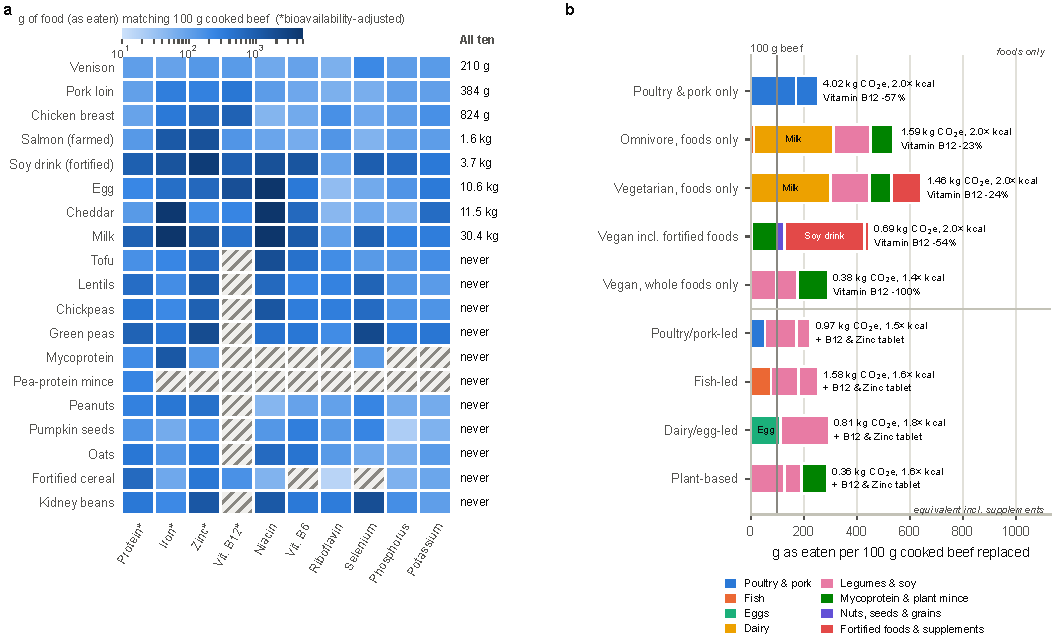
\includegraphics[width=\linewidth]{../figures/fig1_nutrition.pdf}
\caption{\textbf{What it takes to replace the nutrients in 100\,g of cooked beef.} \textbf{a},
Grams of each food (as eaten) that supply the same amount of each nutrient as 100\,g of cooked
lean beef mince. Asterisks mark bioavailability-adjusted nutrients (DIAAS-weighted protein,
absorbable iron, zinc and vitamin~B\textsubscript{12}). Hatched cells: the food contains none of the
nutrient. The right-hand column gives the amount needed to match all ten nutrients at once.
\textbf{b}, Minimum-emission baskets from linear programmes that match the key nutrients
(quality-adjusted protein, absorbable iron, zinc and B\textsubscript{12}, and selenium) within twice
beef's energy, with saturated fat and sodium capped. The upper five use foods only; the lower four
must be fully equivalent and may use B\textsubscript{12} and zinc tablets. Labels give emissions per
100\,g of beef replaced, energy relative to beef, supplements used and any remaining shortfall.}
\label{fig:nutrition}
\end{figure}

Protein is the easy part (\figref{fig:nutrition}a). Chicken breast matches beef's quality-adjusted
protein with \EqChickenProtein{}, tofu with \EqTofuProtein{} and mycoprotein with \EqMycoproteinProtein{}.
Cooked lentils need \EqLentilsProtein{} because their DIAAS is low\cite{nosworthy2017}. Zinc and
vitamin~B\textsubscript{12} are the binding nutrients. Matching beef's absorbable zinc takes \EqChickenZinc{}
of chicken breast, \EqPorkZinc{} of pork loin and \EqLentilsZinc{} of lentils. The phytate in pulses
roughly halves zinc absorption\cite{efsa2014zinc}. The exceptions are mycoprotein (\EqMycoproteinZinc{}),
whose zinc content is high and which contains almost no phytate\cite{finnigan2019,mayerlabba2022},
and pumpkin seeds (\EqSeedsZinc{}, but over 900\,kcal). Vitamin~B\textsubscript{12} occurs naturally only in
animal foods. Matching it takes \EqSalmonBtwelve{} of salmon, \EqMilkBtwelve{} of milk, \EqChickenBtwelve{} of
chicken or \EqEggBtwelve{} of egg, whose B\textsubscript{12} is poorly absorbed\cite{watanabe2007}. It takes
\EqCerealBtwelve{} of fortified cereal, and no amount of any unfortified plant food. Of the nineteen
alternatives, only wild venison (\EqVenisonAll{}) and pork loin (\EqPorkAll{}) match all ten nutrients in
less than half a kilogram. Imperial's own substitutes included venison and pork\cite{imperial2026progress}.

Optimising combinations of foods tells the same story (\figref{fig:nutrition}b, Table~\ref{tab:baskets}).
Using foods alone and staying within twice beef's energy, no diet without ruminant meat matches all
the key nutrients. Poultry and pork alone leave B\textsubscript{12} \BasketMeatSwapShort{}. The best omnivore
basket (salmon, milk, lentils, mycoprotein and fortified cereal) is still short by 23\% and needs
\MinEnergyOmnivore{} times beef's energy to close the gap. Vegetarian and vegan food-only baskets cannot
close it at any energy level given realistic portion caps. Adding a vitamin~B\textsubscript{12} tablet, and
in some cases a small zinc supplement, changes this. All four nutritionally equivalent baskets,
poultry/pork-led, fish-led, dairy/egg-led and plant-based, then match every key nutrient. They use
228--296\,g of food and 1.5--1.8 times beef's energy. For example, the plant-based basket is
\BasketEqVeganDesc{}. These baskets also deliver more fibre, potassium and phosphorus and less saturated fat
than beef. The dairy/egg-led and plant-based baskets supply less niacin and vitamin
B\textsubscript{6}, partly because these are not reported for mycoprotein (Supplementary Table~5).
Both are plentiful in UK diets. The answer to the biological question is therefore qualified. The same
nutrition is obtainable, mainly from pulses, mycoprotein, fish, eggs, dairy and lean meats, but it
takes about two to three times the food mass and 50--80\% more energy. Matching beef's absorbable
B\textsubscript{12} and zinc in practice requires fortified foods or supplements. This is consistent with
the lower zinc and B\textsubscript{12} status observed in vegetarians and vegans\cite{foster2013,neufingerl2022}.

\begin{table}[t]
\centering\footnotesize
\caption{\textbf{Baskets replacing 100\,g of cooked beef.} Minimum-emission solutions with the key
nutrients as targets and energy capped at \LpEnergyMaxRatio{} times beef's. ``kcal $\times$'' is the
basket's energy relative to beef. ``min. kcal $\times$'' is the least energy at which the scenario can
match all key nutrients (``none'': impossible with realistic portions). Beef itself emits
\PerHundredUkAttr{}\,kg \COtwoe{} per 100\,g (UK supply mix).}
\label{tab:baskets}
\begin{tabular}{>{\raggedright\arraybackslash}p{2.3cm}>{\raggedright\arraybackslash}p{6.2cm}rrrl}
\toprule
Scenario & Basket replacing 100\,g cooked beef & kg \COtwoe & kcal $\times$ & min. kcal $\times$ & Largest gap \\
\midrule
Poultry \& pork only & 171\,g chicken breast, 85\,g pork loin & 4.02 & 2.0 & none & B\textsubscript{12} $-$57\% \\
Omnivore, foods only & 300\,g milk, 140\,g lentils, 85\,g mycoprotein, 12\,g salmon, 11\,g fortified cereal & 1.59 & 2.0 & 2.3 & B\textsubscript{12} $-$23\% \\
Vegetarian, foods only & 300\,g milk, 148\,g lentils, 112\,g soy drink, 84\,g mycoprotein, 3\,g fortified cereal & 1.46 & 2.0 & none & B\textsubscript{12} $-$24\% \\
Vegan incl. fortified foods & 300\,g soy drink, 94\,g mycoprotein, 29\,g pumpkin seeds, 20\,g fortified cereal, 5\,g lentils & 0.69 & 2.0 & none & B\textsubscript{12} $-$54\% \\
Vegan, whole foods only & 116\,g mycoprotein, 95\,g kidney beans, 81\,g lentils & 0.38 & 1.4 & none & B\textsubscript{12} $-$100\% \\
\midrule
Poultry/pork-led & 118\,g chickpeas, 54\,g chicken breast, 51\,g lentils, 4\,g mycoprotein, 0.4 zinc tablet, 0.3 b12 tablet & 0.97 & 1.5 & 1.2 & -- \\
Fish-led & 103\,g lentils, 77\,g kidney beans, 76\,g salmon, 0.5 zinc tablet, 0.2 b12 tablet & 1.58 & 1.6 & 1.6 & -- \\
Dairy/egg-led & 184\,g kidney beans, 112\,g egg, 0.4 zinc tablet, 0.3 b12 tablet & 0.81 & 1.8 & 1.6 & -- \\
Plant-based & 126\,g kidney beans, 98\,g mycoprotein, 65\,g chickpeas, 0.3 b12 tablet, 0.1 zinc tablet & 0.36 & 1.6 & 1.3 & -- \\
\bottomrule
\end{tabular}

\end{table}

%=================================================================== results 2
\section{Equivalent nutrition with a tenth of the emissions}

We built the emission factor of beef eaten in the UK from its origin and production system
(Methods; Extended Data Fig.~\ref{fig:ef}). About 72\% of supply is home-produced, roughly half of
it from the dairy herd\cite{defra2025auk,ciel2020}, and most imports come from Ireland. Farm
footprints were taken from UK and FAO data\cite{ciel2020,prism2024,gerber2013} and converted to retail
weight. The result is \EfBeefUkAttr{}\,kg \COtwoe{} per kg of retail beef, close to Poore and Nemecek's
average for UK producers (\EfBeefPnUk{}\,kg) and about half their global average of
\EfBeefPnMix{}\,kg for the same herd mix\cite{poore2018}. A 100\,g portion of cooked beef therefore
carries \PerHundredUkAttr{}\,kg \COtwoe{} (Monte Carlo 90\% interval \PerHundredBeefMc{}). The
nutritionally equivalent baskets carry 0.36--1.58\,kg, even though we deliberately used global mean
footprints for every alternative food, which overstates UK-sourced pulses, poultry and dairy
(\figref{fig:emissions}a). Replacing beef with equivalent nutrition therefore cuts the associated
emissions by \ReductionMin--\ReductionMax\%. The fish-led basket saves least (\PctVsBeefEqFish\%) and
the plant-based basket most (\PctVsBeefEqVegan\%).

\begin{figure}[t]
\centering
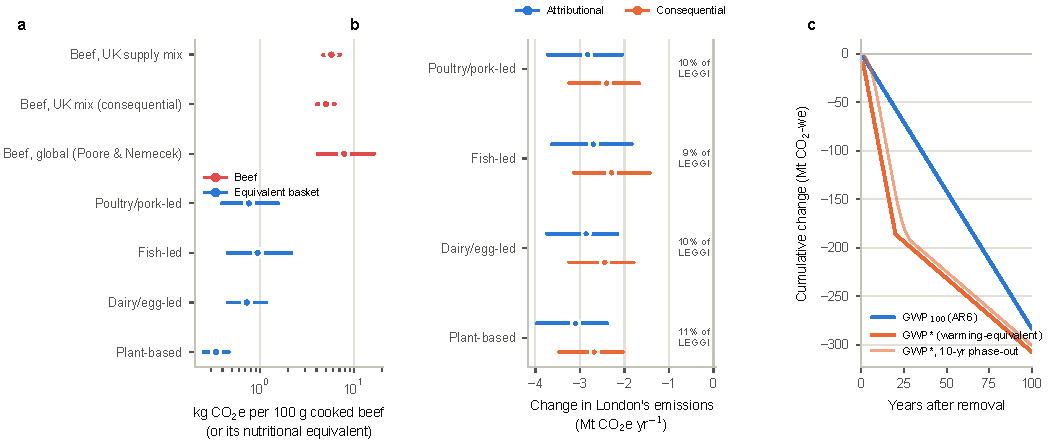
\includegraphics[width=\linewidth]{../figures/fig2_emissions.pdf}
\caption{\textbf{Emissions of beef and of its nutritionally equivalent replacements.}
\textbf{a}, kg \COtwoe{} per 100\,g of cooked beef, or per basket that replaces it. Dots are
Monte Carlo medians and lines 90\% intervals. ``UK supply mix'' combines six origin-by-system
segments; ``global'' uses Poore and Nemecek's distributions for beef- and dairy-herd beef.
\textbf{b}, Annual change in London's emissions if all beef eaten by Londoners were replaced
by each basket. Attributional accounting counts beef's full footprint; consequential accounting
counts only emissions that disappear when demand stops (dairy-origin beef keeps the cow's share).
Text gives the attributional median as a share of London's 2023 territorial inventory (LEGGI).
\textbf{c}, Cumulative change in warming-equivalent emissions after London stops eating beef,
under GWP\textsubscript{100} and under GWP*, which treats methane as a short-lived pollutant.}
\label{fig:emissions}
\end{figure}

Scaling up uses the national supply balance. The UK consumes \CweKg{}\,kg of beef per person
a year in carcass-weight terms\cite{defra2025auk}, which corresponds to \FlowRetail{}\,kg bought
at retail and \FlowEaten{}\,kg eaten cooked (\FlowEatenGDay{}\,g a day). That beef emits \BeefPcKg{}\,kg
\COtwoe{} per person a year. The equivalent baskets save \DeltaPcEqFish--\DeltaPcEqVegan{}\,kg per person,
about \PctDiet\% of an average UK diet's footprint\cite{scarborough2014}. For London's \PopLondonM{}
million residents\cite{ons2025pop}, beef consumption emits \LondonBeefMt{}\,Mt \COtwoe{} a year.
Replacing it with equivalent nutrition would cut emissions by \LondonDeltaMin--\LondonDeltaMax{}\,Mt a
year, or \LondonDeltaMc{}\,Mt for the poultry/pork-led basket including all parameter uncertainty
(\figref{fig:emissions}b). This is equivalent to \PctLeggiMin--\PctLeggiMax\% of London's
\Leggi{}\,Mt territorial inventory for 2023\cite{leggi2025} and \PctCbeMin--\PctCbeMax\% of its
\Cbe{}\,Mt consumption-based footprint\cite{gla2024cbe}. With global-average beef footprints the
saving doubles to \LondonDeltaPnMin--\LondonDeltaPnMax{}\,Mt (\PctLeggiPnMin--\PctLeggiPnMax\% of
LEGGI). Counting only consequential emissions, the saving is \LondonDeltaMcConseq{}\,Mt.
Nationally the change is about \UkDelta{}\,Mt a year, or \PctUkTerr\% of UK territorial emissions.
For comparison, enteric fermentation by UK beef cattle alone emits \UkBeefEnteric{}\,Mt\cite{desnz2026ghg}.
The largest source of uncertainty is how much beef people eat: survey-based intakes are about a
third lower than the supply balance implies\cite{stewart2021} (Extended Data Fig.~\ref{fig:tornado}).

How these numbers should be read matters. The ``percentage of London'' is a comparison of
magnitudes, not a reduction in London's inventory. LEGGI counts emissions inside the city
boundary, and London's livestock emits only about 0.01\,Mt\cite{leggi2025}. Almost all of the saving
would occur on farms in the UK, Ireland and further afield. The consumption-based comparison is
the like-for-like one: equivalent to a 3--4\% cut in everything Londoners' consumption causes, or
about a third of the 9.8\,Mt attributed to their food\cite{gla2024cbe}. The choice of climate metric
also matters, because \BeefGasChFour\% of beef's footprint is methane. Under GWP\textsubscript{20} the saving
doubles (\GwpTwentyDelta{}\,Mt). Under GWP*, which represents the effect of a sustained change in
methane emission rate on warming\cite{cain2019gwpstar,smith2021gwpstar}, removing London's
\LondonChFourKt{}\,kt of annual beef methane gives a cumulative warming-equivalent reduction of
\CumStarTwenty{}\,Mt after 20 years. That is \CumStarRatioTwenty{} times the GWP\textsubscript{100} figure, and the two
converge after a century (\figref{fig:emissions}c). Whether GWP* is appropriate for attributing
responsibility is debated\cite{rogelj2019,lynch2020}, but it shows that ending a methane source buys
near-term cooling. Finally, land freed from beef could store carbon. Searchinger and colleagues'
carbon opportunity cost of 144\,kg \COtwoe{} per kg of beef\cite{searchinger2018} would add roughly
\CocLondonMt{}\,Mt a year for London's consumption. That is far larger than the production emissions,
but realising it requires the freed land to be restored\cite{hayek2021}, so we do not count it in the
headline numbers.

%=================================================================== results 3
\section{A campus ban is diluted by diners and markets}

Taste Imperial bought \FoiBeefTwentyTwo{}\,t of beef in 2022/23 and \FoiBeefTwentyThree{}\,t in 2023/24,
and \FoiBeefTwentyFour{}\,t after removal (freedom-of-information records\cite{imperialfoi};
Supplementary Note~1). At 120\,g per portion this is about \CampusBeefMeals{} beef meals a year. A
procurement inventory would book the removal of \CampusLrGross{}\,t \COtwoe{} a year, minus the
replacement dishes: \CampusLrAcct{}\,t net. That is \CampusPctImperial\% of Imperial's \ImperialTotalKt{}\,kt
footprint\cite{imperial2025annual} and about \CampusPctCatering\% of its catering emissions. Two responses
outside the campus reduce this saving (\figref{fig:campus}).

First, some diners buy beef elsewhere. Evidence from canteens suggests this is small. Beef-free
days at German universities did not change total or main-dish sales\cite{merk2024}. Doubling
vegetarian availability in Cambridge colleges showed no rebound at the evening meal\cite{garnett2019}.
Removing meat options in Oxford left sales at eleven nearby cafeterias unchanged\cite{pechey2022}. By
contrast, whole meat-free days at a Swiss university cut on-campus sales by 17\%\cite{russo2025}. We
assume 7\% of forgone beef meals are bought as beef off campus (Supplementary Table~15), which adds
back \CampusLrOff{}\,t.

Second, and more important, beef that Imperial no longer buys does not simply stay unproduced. In
an integrated market, a fall in demand lowers the price slightly and other buyers absorb part of
the freed supply. Only the share $\phi=\eta/(\eta-\varepsilon)$ of the demand cut reaches production,
where $\eta$ is the supply elasticity and $\varepsilon$ the demand elasticity\cite{alston1995science,norwood2011}.
With UK beef demand elasticity of $-0.59$\cite{tiffin2011} and US-based supply elasticities of about
0.1--0.4 within a year and 1--5 within a decade\cite{usda2015cool,suh2017}, our multi-market
equilibrium model gives a beef pass-through of \CampusPassLr{} in the long run and \CampusPassSr{} in the
short run (\figref{fig:campus}a). The long-run value is close to Norwood and Lusk's widely used
estimate of 0.68\cite{norwood2011}. Market leakage therefore adds back \CampusLrLeak{}\,t in the long
run. Replacement foods add \CampusLrSubs{}\,t, and their own market adjustment removes
\CampusLrSubsAdj{}\,t.

\begin{figure}[t]
\centering
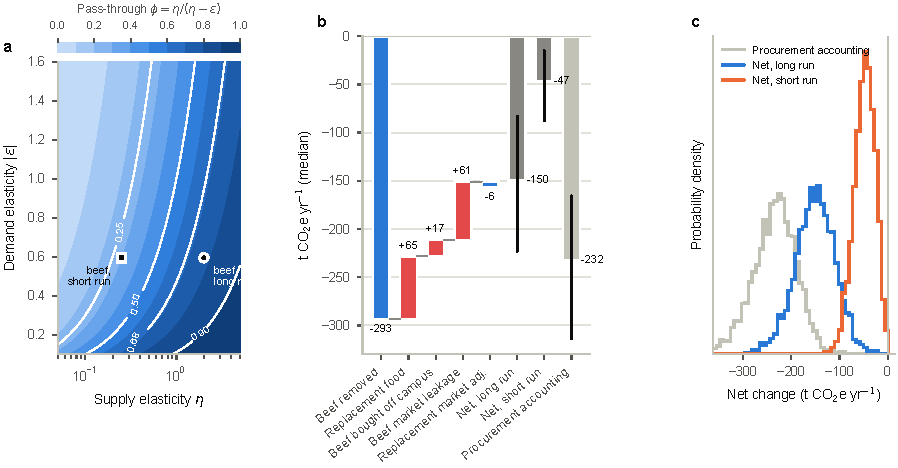
\includegraphics[width=\linewidth]{../figures/fig3_campus.pdf}
\caption{\textbf{From campus purchases to atmospheric emissions.} \textbf{a}, Share of a demand cut
that reaches production, $\phi=\eta/(\eta-\varepsilon)$, as a function of supply ($\eta$) and demand
($\varepsilon$) elasticities. Markers show beef in the short and long run. \textbf{b}, Decomposition of
the annual emissions change from removing beef at Imperial (long-run Monte Carlo medians). Grey
bars show net outcomes, with 90\% intervals, and what procurement accounting would report.
\textbf{c}, Distributions of the net change (\NCampus{} draws).}
\label{fig:campus}
\end{figure}

The net long-run effect is a reduction of \CampusLrNet{}\,t \COtwoe{} a year (90\% interval
\CampusLrNetLo--\CampusLrNetHi{}\,t). This is \CampusNetVsGrossLr\% of the beef's own footprint and
\CampusNetVsAcctLr\% of what the inventory would report. In the first year the reduction is only
\CampusSrNet{}\,t (\CampusSrNetLo--\CampusSrNetHi{}\,t). Because the replacement food's emissions are
about a quarter of the beef's, the ban reduces emissions only if pass-through exceeds
\CampusPhiStar{} (Extended Data Fig.~\ref{fig:campusgrid}). If beef production did not respond at all,
the policy would increase emissions by about \CampusNoResponse{}\,t a year. At city scale the change,
about \CampusPpmLondon{} parts per million of London's territorial emissions, is too small to measure.
Imperial's own records illustrate a further difficulty for evaluation. Chicken and pork purchases
were already rising by about 12\,t and 2\,t a year before the ban, and they kept rising afterwards
(\FoiChickenTwentyFour{}\,t and \FoiPorkTwentyFour{}\,t in 2024/25). The emissions embodied in all meat
purchases fell from \FoiMeatTTwentyThree{}\,t to \FoiMeatTTwentyFour{}\,t, but a before--after comparison
would mix the policy with these trends (Supplementary Note~12).

%=================================================================== results 4
\section{What the ban costs diners, and what it does to their diets}

With food prices held fixed, the only change for diners is a smaller choice set. In a random-utility
model of dish choice, removing an option lowers each diner's expected utility by a log-sum
amount\cite{small1981,train2009}. We calibrate the model to a beef-dish own-price elasticity of about
$-1.5$\cite{garnett2021,salvi2025} and beef's \PBeefPct\% share of main meals. The loss per forgone beef
meal is then \WelfareLossMeal{} (\figref{fig:students}a). Calibrated this way, the loss is almost
exactly the meal price divided by the dish elasticity, whatever the strength of substitution
within the meat nest (Supplementary Note~10). Because diners can always buy beef off campus, we
also cap the loss at the cost of doing so, which gives \WelfareLossMealCapped{} per meal. Across
\CampusBeefMeals{} beef meals the annual welfare loss is \WelfareLossCappedTotal{} (capped). The
monetised climate benefit, at the UK's central carbon value of £\CarbonValue{} per tonne
\cite{desnz2023carbon}, is \BenefitTotal{} (\figref{fig:students}b). The implied cost is \CostPerT{} per
tonne avoided (capped: \CostPerTCapped{}). The welfare loss exceeds the climate benefit in essentially
all Monte Carlo draws. The ban would break even only if diners valued a beef meal at no more than
£\BreakEvenLossMeal{} over their next-best option.

\begin{figure}[t]
\centering
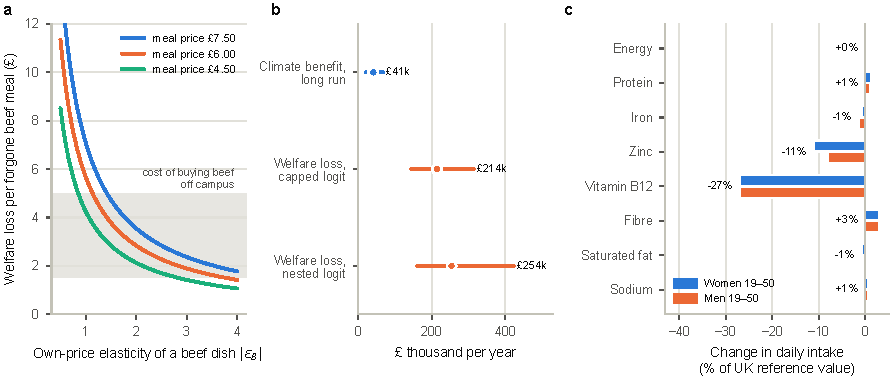
\includegraphics[width=\linewidth]{../figures/fig4_students.pdf}
\caption{\textbf{Consequences for diners.} \textbf{a}, Welfare loss per forgone beef meal from a
nested-logit model calibrated to the own-price elasticity of a beef dish, for three meal prices.
The grey band is the cost of buying beef off campus instead, which caps the loss. \textbf{b},
Annual welfare loss with prices held fixed, compared with the monetised long-run climate benefit
at the UK central carbon value (medians and 90\% intervals). \textbf{c}, Change in average daily
intake for someone who ate beef on campus \FreqMeals{} times a week, expressed as a share of UK
reference values (RNI; fibre target; maximum for saturated fat and sodium).}
\label{fig:students}
\end{figure}

This welfare estimate should be read as an upper bound on private cost rather than a verdict. It
ignores habit formation, which erodes the loss over time. It ignores any value diners place on
eating more sustainably. It also ignores health benefits of eating less red meat that diners do
not fully take into account. All three can be measured (Supplementary Note~12). It is nonetheless
consistent with other evidence that bans are a costly way to change diets: a one-off climate
lecture reduced students' meat consumption for three years at about US\$14 per tonne\cite{jalil2023},
and carbon labels\cite{lohmann2022} and more vegetarian options\cite{garnett2019,becker2026} reduce
emissions while keeping choice.

The nutritional consequences for diners are small on average but not for everyone
(\figref{fig:students}c). Each forgone beef meal, replaced by Imperial's observed mix of chicken,
pork, venison, fish, vegetarian and vegan dishes, provides \DeltaProteinMeal{}\,g more protein and
\DeltaFibreMeal{}\,g more fibre. It provides \DeltaZincMeal{}\,mg less zinc, \DeltaBtwelveMeal{}\,\textmu g less
vitamin~B\textsubscript{12} and \DeltaIronMeal{}\,mg less iron. For a student who ate beef on campus
\FreqMeals{} times a week, that means \FreqZincWomen\% less zinc and \FreqBtwelve\% less B\textsubscript{12} relative
to the reference intakes for women. These deficits are worth monitoring in groups whose iron and
zinc intakes are already marginal\cite{ndns2020}. Averaged over Imperial's \CampusPeople{} students and
staff, the zinc deficit is only \PopAvgZinc{}\,mg a day.

%=================================================================== discussion
\section{Implications}

Our results separate two claims that are often merged. The first is that replacing beef with
other foods cuts emissions, and this is robust. The cut is 72--93\% per portion when nutrition is
matched, and it holds whichever basket is chosen and whether UK or global footprints are used. A
city the size of London would avoid emissions equivalent to roughly a tenth of its territorial
inventory, and even more under short-horizon metrics. The second claim is that a single institution
achieves that cut by removing beef from its menus. This is much weaker. Market leakage, off-campus
purchases and the emissions of substitute food cut the net saving to about half of the beef's
footprint in the long run and about a sixth in the first year. A campus can report a large reduction in its procurement inventory while
the effect on the atmosphere is smaller and, without a market response, could even be positive.
This is the consequential-LCA point that a purchaser's inventory does not show the marginal effect
of its decisions\cite{ekvall2004,budolfson2019}.

Three practical conclusions follow for Imperial and similar institutions. First, nutrition: removing
beef should come with appealing zinc- and B\textsubscript{12}-rich alternatives. Mycoprotein, pulses with
vitamin~C, fish, eggs, dairy and fortified foods all qualify, and the mycoprotein and venison dishes
Imperial already serves are good choices on these measures. Clear guidance on vitamin~B\textsubscript{12}
is needed for students who stop eating meat. Second, accounting: claims should report consequential
estimates alongside procurement inventories, with the short-run pass-through made explicit. Third,
evaluation: the policy's effects on diets, satisfaction and welfare can be measured with till data,
repeated 24-hour recalls\cite{bradley2016}, biomarkers and discrete-choice experiments\cite{johnston2017}.
Estimates should use designs that account for pre-existing trends\cite{callaway2021,abadie2010,hausman2018}
(Supplementary Note~12). Detecting a change in zinc intake of 0.5\,mg a day needs about \PowerN{}
participants per group, so studies must target frequent campus diners.

Our analysis has limitations. Nutrient equivalence is assessed per portion against one reference
cut (lean mince). Bioavailability uses food-level absorption factors rather than meal-level models,
and complementary proteins in mixed baskets are not credited. Emission factors for alternatives are
global means, and market elasticities come from US and UK studies of whole national markets. The
welfare model assumes the logit structure, and the dish elasticity that drives it has not been
measured on any UK campus. Each assumption is exposed in the open code and data, and the
Supplementary Information traces every number from its source to the result.

%===================================================================== methods
\section{Methods}

\subsection{Overview and reproducibility}
The model is written in Python (NumPy, SciPy, pandas). All inputs are in plain-text files in the
repository's \texttt{data/} folder, each annotated with its source. One script reruns every
calculation, writes all figures and tables, and generates the numbers quoted in this paper as LaTeX
macros, so the text cannot drift from the code. Supplementary Information Notes~1--13 give every
equation, parameter and intermediate result. Uncertainty is propagated by Monte Carlo simulation
(\NMC{} draws for London, \NCampus{} for the campus); we report medians with 90\% intervals.

\subsection{Food composition and bioavailability}
Nutrient contents per 100\,g as eaten were taken from USDA FoodData Central SR Legacy\cite{usdafdc}
for 16 foods (FDC identifiers in Supplementary Table~3), from manufacturer labels and analyses for
mycoprotein\cite{finnigan2019,mayerlabba2022} and plant-based mince, and from UK labels for fortified
cereal and soya drink. The reference is 90\%-lean beef mince, pan-browned. Protein is weighted by
truncated DIAAS from pig and rat assays\cite{fao2013protein,bailey2020,mathai2017,han2020,nosworthy2017,rutherfurd2015,reynaud2021}.
Iron is split into haem and non-haem pools absorbed at 25\% and 10\%\cite{efsa2015iron,hurrell2010}. Zinc
absorption is 35\% from animal foods, 25\% from moderate-phytate foods and 18\% from pulses, seeds and
whole grains\cite{fao2004vitmin,izincg2004,efsa2014zinc}. Vitamin~B\textsubscript{12} absorption is 60\% from meat,
42\% from fish, 65\% from dairy, 9\% from eggs and 50\% from fortificants\cite{watanabe2007}. Ranges
for all factors are tested in sensitivity analyses. UK reference nutrient intakes follow COMA\cite{dh1991}.

\subsection{Single-food equivalents and diet optimisation}
For food $i$ and nutrient $k$, the mass matching 100\,g of beef is $100\,b_k/a_{ik}$, where $b_k$ is beef's
content and $a_{ik}$ the food's. Baskets are found by linear programming (HiGHS via SciPy). The
programme minimises emissions subject to: supply of each key nutrient at least equal to beef's; energy
between 0.85 and \LpEnergyMaxRatio{} times beef's; saturated fat no higher than beef's; sodium no more than
\LpSodiumAllow{}\,mg above beef's; and portion caps. Each nutrient constraint has a penalised slack
variable, so unavoidable shortfalls are reported rather than making the problem infeasible. Scenarios
restrict the allowed food groups. ``Equivalent'' scenarios also require at least 60\% (dairy/egg-led:
50\%) of quality-adjusted protein to come from the named group and allow B\textsubscript{12} and zinc tablets.
A minimum-energy variant gives the least energy at which each scenario can match beef. Sensitivity
analyses cover bioavailability (plant-favourable and plant-unfavourable extremes), no bioavailability
adjustment, a strict $\pm$15\% energy band, and matching all ten nutrients (Extended Data Fig.~\ref{fig:basketsens}).

\subsection{Emission factors}
For alternative foods we use Poore and Nemecek's global mean emissions per kg of retail product as
central values and their 5th, 50th and 95th percentiles to fit log-normal distributions\cite{poore2018}.
For foods they do not cover we use verified product footprints: mycoprotein\cite{quorn2024} and
plant-based mince\cite{heller2018,gfi2021}. Cooking yields come from USDA and Bognár tables\cite{showell2012,bognar2002},
and a household waste fraction of \WastePct\% applies to all foods\cite{defra2010waste}. For beef we combine
six supply segments: UK suckler, UK dairy-origin, Ireland, other Europe, Oceania and South America
(Supplementary Table~8). Their shares come from Defra supply statistics and import data\cite{defra2025auk}.
Farm-gate footprints per kg of carcass come from Defra/CIEL, PRISM (Agrecalc) and FAO GLEAM data\cite{ciel2020,prism2024,gerber2013}.
These are converted to retail weight with a yield of \RetailYield{} and a post-farm-gate adder of
\PostFarm{}\,kg \COtwoe{} per kg. In the consequential variant, dairy-origin beef carries only the rearing
and finishing share of its footprint (avoidable fraction 0.7), because the cow's emissions are
reallocated to milk rather than avoided\cite{ekvall2004}.

\subsection{Scaling, metrics and Monte Carlo}
Per-capita beef supply (\CweKg{}\,kg carcass weight a year; production plus imports minus exports divided
by population\cite{defra2025auk,ons2025pop}) is converted to retail purchases and cooked intake as above.
Annual emission changes are $10\,B_{\mathrm{eaten}}\mathrm{GHG}_b - B_{\mathrm{retail}}\mathrm{EF}_{\mathrm{beef}}$
per person and are scaled by London's and the UK's populations. They are compared with LEGGI 2023
(territorial)\cite{leggi2025}, London's consumption-based footprint for 2022\cite{gla2024cbe} and UK national
totals\cite{desnz2026ghg}. Metric conversions use each footprint's gas composition and the GWP vintage
in which it was reported, converted to AR6 values\cite{forster2021ar6}. Warming-equivalent emissions use
GWP* with the coefficients of Smith et al.\cite{smith2021gwpstar}. The Monte Carlo samples consumption,
yields, waste, segment footprints, segment shares (Dirichlet), avoidable fractions and every
alternative-food footprint jointly. One-at-a-time sensitivities are shown in Extended Data Fig.~\ref{fig:tornado}.

\subsection{Market model}
The campus shock is propagated through an equilibrium displacement model of nine UK food markets
(beef, lamb, pork, poultry, fish, eggs, dairy, plant protein and venison)\cite{alston1995science,wohlgenant1993}.
Each market has constant-elasticity supply and demand with own- and cross-price elasticities. A
demand shift $\Delta D$ at constant prices changes prices by $(\mathrm{diag}(\eta)-\mathcal{E})^{-1}\Delta D/Q$
and production by $Q\eta\,\mathrm{d}\ln P$ (Supplementary Note~9). Demand elasticities come from UK
estimates and meta-analyses\cite{tiffin2011,andreyeva2010,gallet2010}, including UK cross-price
elasticities among meats\cite{tiffin2011}. Short-run (1-year) and long-run (10-year) supply elasticities
come from US estimates\cite{usda2015cool,suh2017}, moderated for an integrated European market, and are
sampled from triangular distributions (Supplementary Table~11). The shock is built from Imperial's
beef purchases (\CampusBeefT{}\,t a year, freedom-of-information data\cite{imperialfoi}), the share of
forgone beef meals going to each alternative dish type or off campus (Dirichlet-distributed;
Supplementary Table~15), and dish recipes. Beef uses the consequential emission factor
(\CampusEfConseq{}\,kg \COtwoe{} per kg).

\subsection{Welfare and nutrient intake of diners}
Diners choose dishes in a nested logit with beef and other meat dishes in one nest (dissimilarity
$\lambda$). With prices fixed, the compensating variation per meal occasion is
$\ln\!\left(1-P_M+P_M(1-P_B/P_M)^{\lambda}\right)/\alpha$\cite{small1981,train2009}. The marginal utility of
money $\alpha$ is calibrated so that the beef dish's own-price elasticity equals $\varepsilon_B$. The loss per
forgone beef meal is capped at the cost of buying beef off campus. Losses are compared with the
avoided emissions valued at DESNZ carbon values (£\CarbonValueLow--\CarbonValueHigh{} per tonne, central
£\CarbonValue{}; 2022 prices)\cite{desnz2023carbon}. Nutrient changes per forgone beef meal use the same
dish recipes and composition data.

\subsection{Use of AI tools}
The analysis code, data assembly and manuscript drafting were carried out with the assistance of
an AI system (Claude, Anthropic). Every numerical input is traceable to the sources cited in the
data files, and the author is responsible for the content.

%================================================================ end matter
\section{Data availability}
All input data, with sources, and all generated results are in the accompanying repository
(\texttt{data/}, \texttt{results/}). The FOI purchase records are published by Imperial College London\cite{imperialfoi}.

\section{Code availability}
The code that reproduces every figure, table and number is in the repository (\texttt{src/beefwhatif},
\texttt{scripts/run\_all.py}) under the MIT licence.

\section{Competing interests}
The author declares no competing interests.

\bibliographystyle{naturemag}
\bibliography{references}

%============================================================== extended data
\clearpage
\setcounter{figure}{0}
\setcounter{table}{0}
\captionsetup[figure]{name=Extended Data Fig.}
\captionsetup[table]{name=Extended Data Table}
\section{Extended Data}

\begin{figure}[H]
\centering
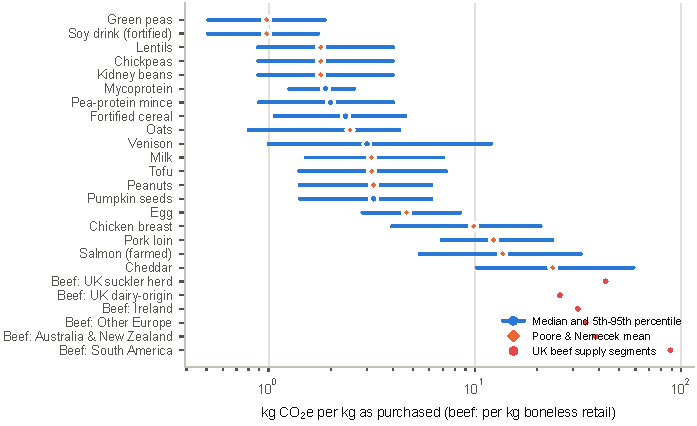
\includegraphics[width=0.7\linewidth]{../figures/ed1_emission_factors.pdf}
\caption{\textbf{Emission factors.} kg \COtwoe{} per kg of each food as purchased: median and
5th--95th percentile range used in the Monte Carlo, with Poore and Nemecek's global means. Red
dots: retail emission factors of the six UK beef supply segments; their consumption-weighted mean
is \EfBeefUkAttr{}\,kg \COtwoe{} per kg.}
\label{fig:ef}
\end{figure}

\begin{figure}[H]
\centering
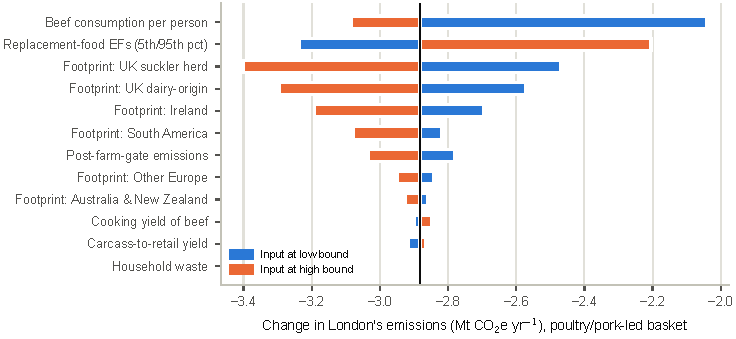
\includegraphics[width=0.75\linewidth]{../figures/ed2_tornado.pdf}
\caption{\textbf{Sensitivity of London's emissions change.} Each input is moved to its low and
high bound with all others at central values (poultry/pork-led basket, UK supply mix). Beef
consumption per person dominates. Its low bound reproduces survey-based intakes.}
\label{fig:tornado}
\end{figure}

\begin{figure}[H]
\centering
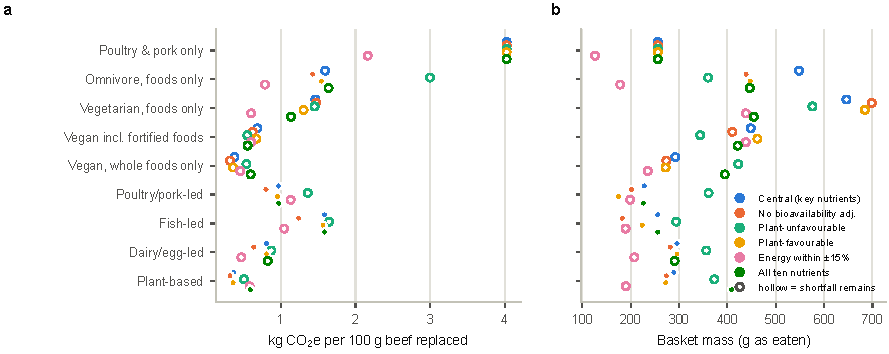
\includegraphics[width=0.85\linewidth]{../figures/ed3_basket_sensitivity.pdf}
\caption{\textbf{Robustness of the optimised baskets.} \textbf{a}, Emissions and \textbf{b}, mass of
each scenario's basket under alternative bioavailability assumptions, a strict isocaloric
constraint and matching all ten nutrients. Hollow markers: a shortfall remains.}
\label{fig:basketsens}
\end{figure}

\begin{figure}[H]
\centering
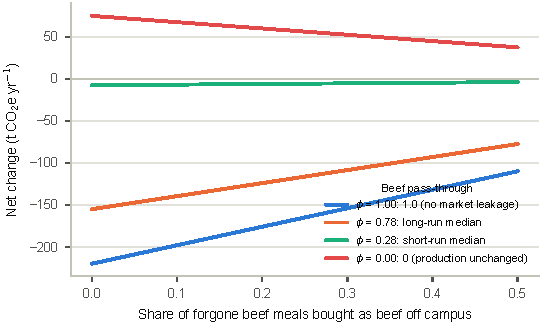
\includegraphics[width=0.62\linewidth]{../figures/ed4_campus_grid.pdf}
\caption{\textbf{Campus net change, beef pass-through and off-campus purchasing.} Net annual change
for Imperial as the share of forgone beef meals bought as beef off campus varies, for
pass-through values from 0 to 1. The sign depends on pass-through alone: the ban reduces emissions
only if pass-through exceeds the ratio of replacement-food to beef emissions (about \CampusPhiStar{}).}
\label{fig:campusgrid}
\end{figure}

\begin{table}[H]
\centering\small
\caption{\textbf{Decomposition of the campus emissions change (t \COtwoe{} yr$^{-1}$).} Monte Carlo
median and 90\% interval.}
\begin{tabular}{lrrr}
\toprule
Component & Long run & Short run & Long run, no cross-price \\
\midrule
Beef removed from menus & \textminus 293 (\textminus 373 to \textminus 233) & \textminus 294 (\textminus 374 to \textminus 233) & \textminus 293 (\textminus 373 to \textminus 236) \\
Replacement food bought & 65 (42 to 103) & 64 (41 to 103) & 64 (43 to 104) \\
Beef bought off campus & 17 (3 to 51) & 18 (3 to 51) & 18 (3 to 51) \\
Beef market leakage & 61 (35 to 109) & 197 (148 to 261) & 61 (36 to 111) \\
Replacement market adjustment & \textminus 6 (\textminus 14 to \textminus 0) & \textminus 36 (\textminus 63 to \textminus 21) & \textminus 12 (\textminus 20 to \textminus 7) \\
\midrule
\textbf{Net change} & \textminus 150 (\textminus 223 to \textminus 83) & \textminus 47 (\textminus 88 to \textminus 15) & \textminus 154 (\textminus 224 to \textminus 94) \\
\midrule
Procurement accounting & \textminus 232 (\textminus 314 to \textminus 165) & \textminus 233 (\textminus 316 to \textminus 166) & \textminus 232 (\textminus 312 to \textminus 168) \\
Beef pass-through $\phi$ & 0.78 (0.62 to 0.87) & 0.28 (0.18 to 0.38) & 0.78 (0.62 to 0.86) \\
\bottomrule
\end{tabular}

\end{table}

\begin{table}[H]
\centering\small
\caption{\textbf{Welfare and monetised climate effects for Imperial diners.}}
\begin{tabular}{lrr}
\toprule
Quantity & Median & 90\% interval \\
\midrule
Loss per forgone beef meal, nested logit (£) & 3.25 & 2.09 to 5.35 \\
Loss per forgone beef meal, capped (£) & 2.75 & 1.92 to 3.92 \\
Annual welfare loss, nested logit (£) & 253{,}969 & 160{,}709 to 423{,}618 \\
Annual welfare loss, capped (£) & 214{,}059 & 144{,}507 to 314{,}739 \\
Emissions avoided, long run (t \COtwoe) & 150 & 83 to 223 \\
Monetised climate benefit (£) & 40{,}818 & 20{,}608 to 68{,}436 \\
Welfare cost per tonne avoided (£/t) & 1{,}730 & 911 to 3{,}725 \\
Welfare cost per tonne, capped (£/t) & 1{,}444 & 818 to 2{,}896 \\
P(capped loss $>$ climate benefit) & 100\% &  \\
\bottomrule
\end{tabular}

\end{table}

\end{document}
